\chapter{MiCS Implementation}

\section{Types in MiCS} % (fold)
\label{sec:types_in_mics}
	To help understand the core type validation and type mapping in general its beneficial to realise the different kind of types that are utilized in MiCS.

	\begin{figure}[H]
		\begin{center}
			\centerline{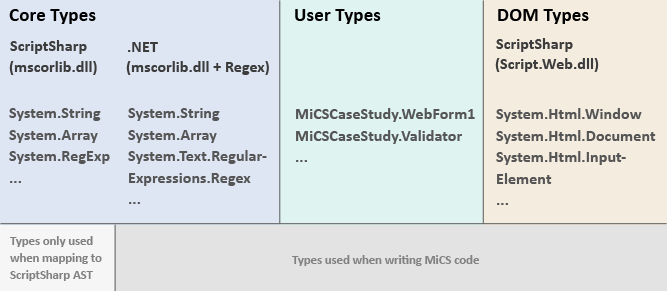
\includegraphics[width=16cm]{resources/images/TypesOverview.png}}
		\end{center}
		\caption{Illustrates the different types used by MiCS.}
		\label{typesOverview}
	\end{figure}

	\subsection{Core Types} % (fold)
	\label{sub:core_types}
		To build the ScriptSharp AST correctly the ScriptSharp core types are required to be associated to the ScriptSharp AST nodes. Their interface is defined to only have features that ScriptSharp can mirror when generating JavaScript which enables full compile time validation. Furthermore the ScriptSharp core types define their equivalent script name (in the class attributes) that is used by the ScriptSharp script generator. An example is the System.Char type (see figure \ref{char}) which is converted to the JavaScript String type as no JavaScript Char type exists.

	\begin{figure}[H]
		\begin{center}
			\centerline{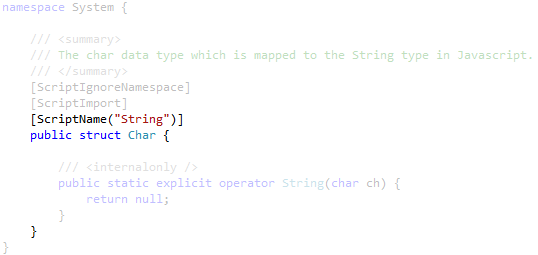
\includegraphics[width=13cm]{resources/images/Char.png}}
		\end{center}
		\caption{The core type System.Char defined in the Script\# mscorlib.dll.}
		\label{char}
	\end{figure}
	% subsection core_types (end)

	\subsection{User Types} % (fold)
	\label{sub:user_types}
		...
	% subsection user_types (end)

	\subsection{DOM Types} % (fold)
	\label{sub:dom_types}
		...
	% subsection dom_types (end)

% section types_in_mics (end)

\section{Syntax Tree Validation} % (fold)
\label{sec:syntax_tree_validation}
	sdsadq qdqw qwd qwd qw 

	\subsection{Mixed Side Principle} % (fold)
	\label{sub:mixed_side_principle}
		sdsadq qdqw qwd qwd qw 
	% subsection mixed_side_principle (end)

% section syntax_tree_validation (end)

\section{Mapping to ScriptSharp AST} % (fold)
\label{sec:mapping_to_scriptsharp_ast}
	When converting the validated Roslyn AST to the ScriptSharp AST we have made a logical division of the process. First the actual mapping from one Roslyn AST node to the equivalent ScriptSharp AST node. Secondly building the ScriptSharp AST from all the mapped nodes. The mapping is discussed in this section. 

	\subsection{Mapping to ScriptSharp Expressions, Statements and Symbols} % (fold)
	\label{sub:subsection_mapping_to_scriptsharp_expressions_statements_and_symbols}
		The mapping of Expressions, Statements and Symbols is implemented in three classes (ExpressionMapper.cs, StatementMapper.cs and SymbolMapper.cs). The three classes are logically divided (and named) after the type of ScriptSharp AST object they map to. 

		\begin{figure}[H]
			\begin{center}
				\centerline{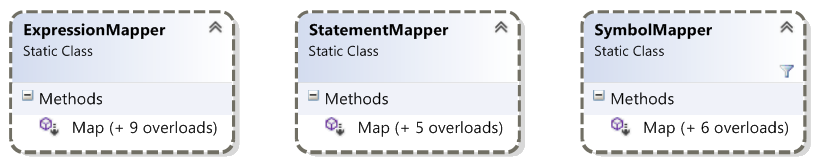
\includegraphics[width=14cm]{resources/images/MapperClasses.png}}
			\end{center}
			\caption{Classes that define extension methods for mapping Roslyn AST nodes to Script\# AST nodes.}
			\label{mapperClasses}
		\end{figure}

		The mapping of the AST nodes is somewhat straightforward as most of the mappings we have done the Roslyn AST maps one to one with the ScriptSharp AST. So a Roslyn return statement node maps to a ScriptSharp return statement etc. The three classes define Map(...) extension methods to the Roslyn objects they map from (see example figures \ref{returnStatementMap} and \ref{conditionaleExpressionMap}).

		\begin{figure}[H]
			\begin{center}
				\centerline{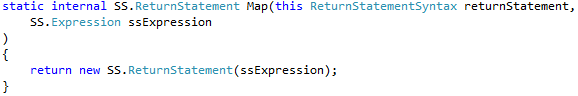
\includegraphics[width=14cm]{resources/images/ReturnStatementMap.png}}
			\end{center}
			\caption{Extension method that maps Roslyn return statement to Script\# return statement.}
			\label{returnStatementMap}
		\end{figure}

		\begin{figure}[H]
			\begin{center}
				\centerline{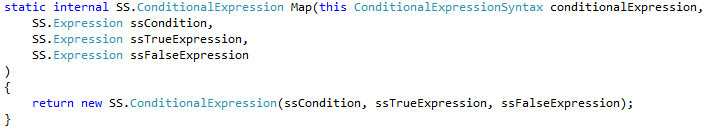
\includegraphics[width=14cm]{resources/images/ConditionalExpressionMap.png}}
			\end{center}
			\caption{Extension method that maps Roslyn conditional expression to Script\# conditional expression.}
			\label{conditionaleExpressionMap}
		\end{figure}
	% subsection subsection_mapping_to_scriptsharp_expressions_statements_and_symbols (end)

	\subsection{Type Mapping} % (fold)
	\label{sub:type_mapping}
		In contrast to using ScriptSharp in the original manner (where the ScriptSharp core types are used when writing code instead of the .NET core types) our project only uses the ScriptSharp core types when mapping to the ScriptSharp JavaScript AST. For this reason the ScriptSharp core types are handled by its own type manager class (ScriptSharpTypeManager.cs). The ScriptSharp core types’ source code are loaded into their own SemanticModel on the TypeManager class. From here the (Roslyn) TypeSymbols are retrieved before they are mapped to ScriptSharp TypeSymbols needed when building the ScriptSharp AST.

		Since the .NET core types are used when writing MiCS code and since these are mapped to the ScriptSharp core types a mapping specification is needed. To facilitate this mapping we have created some simple classes to hold the specification (MiCSCoreMapping.cs, MiCSCoreTypeMapping.cs and MiCSCoreMemberMapping.cs) which then can queried using LINQ. This mapping specification contains information on the core types that we currently support. So if a core type is not described in the specification then it is not supported. If the core type is found in the specification then the same pattern applies for its members. If a type member is not found then it is not supported. The mapping specification also holds information on a member’s return type, number of arguments and the arguments’ types.

		\begin{figure}[H]
			\begin{center}
				\centerline{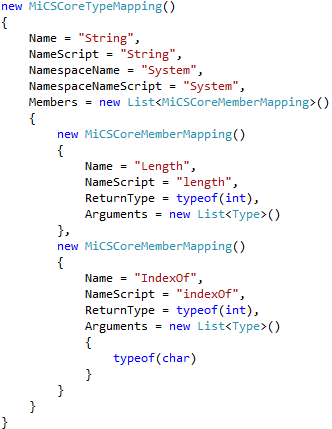
\includegraphics[width=10cm]{resources/images/InitiationOfTypeMapping.png}}
			\end{center}
			\caption{Instantiation example of a single core type (System.String) mapping specification.}
			\label{coreTypeMapping}
		\end{figure}

		An example of a core type mapping is the C\# System.String (see figure \ref{coreTypeMapping}) type which is mapped to the ScriptSharp defined System.String. We are only mapping two of the String type’s members. The field Length which is mapped to the ScriptSharp String type’s Length field (which is the equivalent of the JavaScript String object property length). The second member we map is the IndexOf(Char char) method that returns an int. There are other IndexOf methods that take multiple arguments or a single argument of a different type (than Char) but these are not mapped in our mapping specification.
	% subsection type_mapping (end)
% section mapping_to_scriptsharp_ast (end)

\section{Building the ScriptSharp AST} % (fold)
\label{sec:building_the_scriptsharp_ast}
	... 
	\begin{figure}[H]
		\begin{center}
			\centerline{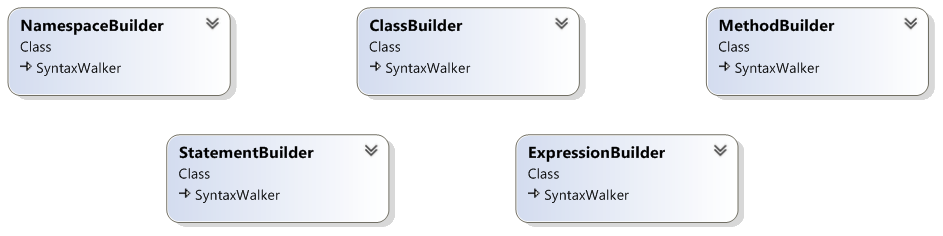
\includegraphics[width=16cm]{resources/images/BuilderClasses.png}}
		\end{center}
		\caption{Classes that built the Script\# AST by traversing the Roslyn AST and utilizing Map(...) extension methods.}
		\label{builderClasses}
	\end{figure}
% section building_the_scriptsharp_ast (end)

\section{Script Generation} % (fold)
\label{sec:script_generation}
	Script generation is done using the ScriptSharp infrastructure only. Specifically the TypeGenerator class located in the ScriptSharp.Generator namespace is utilized for this. The MiCSManager is responsible for instantiating the TypeGenerator and providing it with the ScriptSharp JavaScript AST type nodes (this happens in the MiCSManager.GenerateScriptText method). The ScriptSharp JavaScript AST consists only of the user defined script types.
% section script_generation (end)

\section{Integration with Web Forms} % (fold)
\label{sec:integration_with_web_forms}
	sdsadq qdqw qwd qwd qw 
% section integration_with_web_forms (end)
